% -*- coding: utf-8; -*-

\chapter{Geração Baseada em Derivadas Médias}
\label{ch:my}
	Este capítulo descreve o método proposto nessa dissertação para gerar funções de transferência automáticas, baseado no trabalho de \textit{Kindlmann e Durkin}~\cite{gordon}, explicado no capítulo anterior.

\section{Detecção de Fronteiras}
\label{sec:my.deriv}
	Para eliminar o problema de deslocamento em $ h(v) $ é preciso repensar o modelo de \textit{Kindlmann e Durkin}~\cite{gordon} a fim de identificar a fronteira pela segunda derivada que não seja através de $ f''(x) = 0 $. Uma opção é utilizar o ponto de inflexão que ocorre quando $ f''(x) = 0 $. No entanto, como são encontrados três pontos de inflexão ao longo de $ f''(x) $, é preciso identificar aquele que ocorre quando $ f'(x) $ é máximo.
	
	Para encontrar o ponto de inflexão de uma função, deve-se avaliar sua primeira e segunda derivadas. Na verdade, um ponto de inflexão é encontrado da mesma forma que a fronteira é identificada: um extremo local na primeira derivada e segunda derivada igual a zero. O que faz sentido, uma vez que segundo o modelo estipulado, o centro de uma fronteira é exatamente um ponto de inflexão. A Figura~\ref{fig:m_inflection} mostra $ f''(x) $ como $ D(x) $ e suas respectivas derivadas $ D'(x) $ e $ D''(x) $, onde os pontos de inflexão são indicados pelas retas tracejadas.
	
\begin{figure}[h]
	\centering
	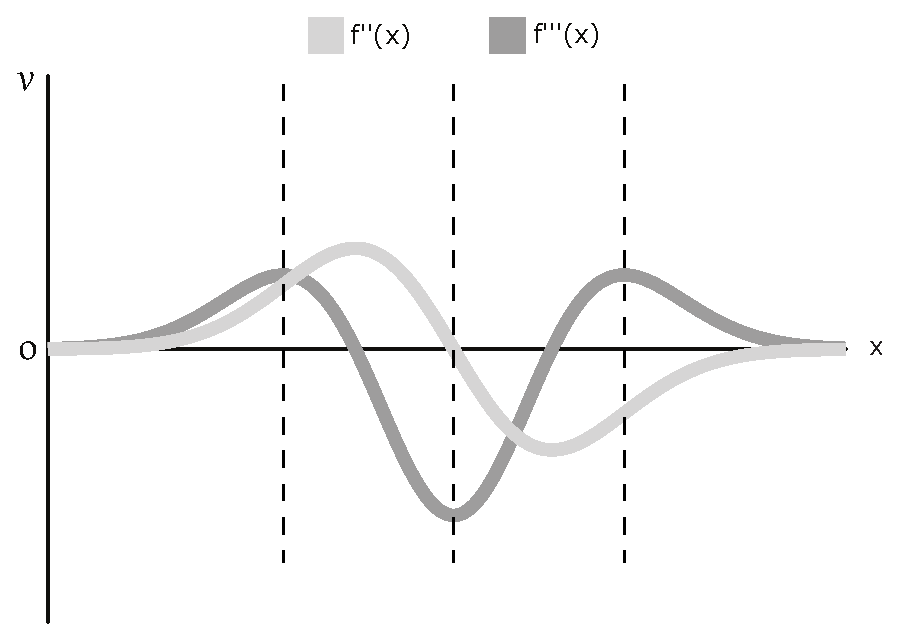
\includegraphics[width=0.7\textwidth]{images/m_inflection}
	\label{fig:m_inflection}
	%TODO
	\caption{Lalala...}
\end{figure}

	Vê-se que apenas um extremo de $ D'(x) $ é negativo. Essa informação é indiferente para encontrar os pontos de inflexão, mas é muito útil na detecção da fronteira, pois a posição do extremo negativo é justamente $ D(x) = 0 $, onde se encontra o centro da fronteira. Lembrando que $ D'(x) = f'''(x), $ percebe-se que $ f'''(x) $ pode ser utilizada no lugar de $ f''(x) $ para identificar uma fronteira, como mostra a Figura~\ref{fig:m_functions}.
	
\begin{figure}[h]
	\centering
	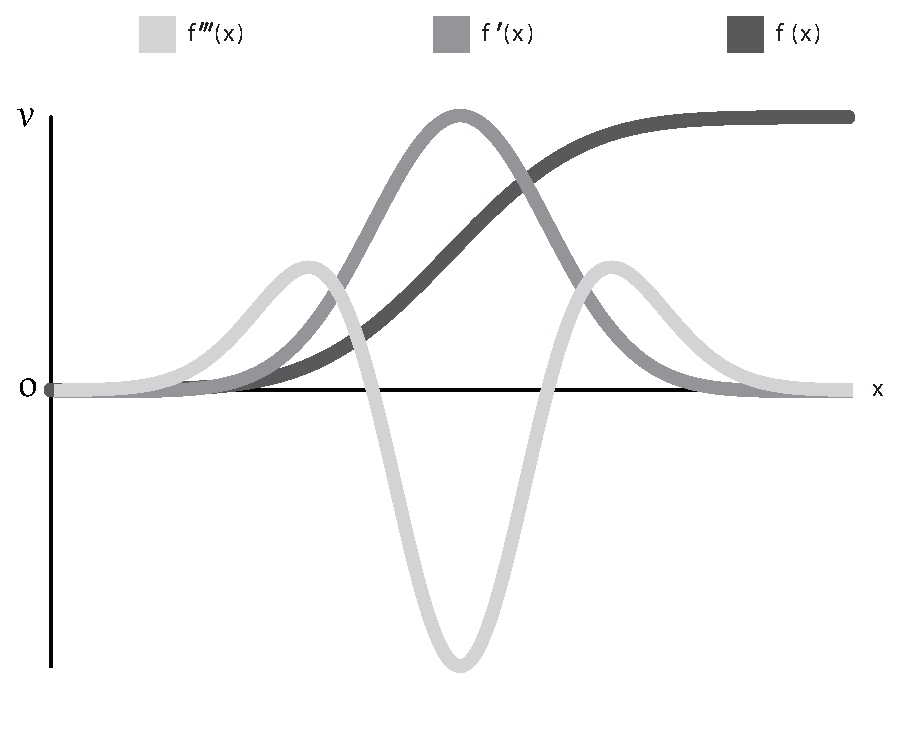
\includegraphics[width=0.7\textwidth]{images/m_functions}
	\label{fig:m_functions}
	%TODO
	\caption{Lalala...}
\end{figure}

	É preciso obter uma nova relação para extrair $ \sigma $ e $ x $, mas agora utilizando $ f'(x) $ e $ f'''(x) $. Para facilitar a leitura, $ f'(x) $ é repetida na equação~\eqref{eq:first2}, enquanto a função $ f'''(x) $ é definida na equação~\eqref{eq:third}. Devido ao fato de $ f'(x) $ ter um grande termo em comum com $ f'''(x) $, a simples divisão entre essas funções revela uma relação envolvendo $ \sigma $ e $ x $, como mostra a equação~\eqref{eq:sigmax}. Com $ x = 0 $ percebe-se que, mais uma vez, o valor de $ \sigma $ pode ser recuperado através dos valores extremos das derivadas, indicado na equação~\eqref{eq:sigma3}. Por fim, $ x $ pode ser isolado na equação~\eqref{eq:sigmax} resultando em uma nova expressão para a distância ao centro da fronteira, indicada na equação~\eqref{eq:x3}.
	\
	
\begin{equation} \label{eq:first2}
	g = f'(x) = \frac{v_{max} - v_{min}}{\sigma\sqrt{2\pi}}\ e^{-\frac{x^{2}}{2\sigma^{2}}}
\end{equation} \
	
\begin{equation} \label{eq:third}
	t = f''(x) = -\frac{(x^{2} - \sigma^{2})(v_{max} - v_{min})}{\sigma^{5}\sqrt{2\pi}}\ e^{-\frac{x^{2}}{2\sigma^{2}}}
\end{equation} \

\begin{equation} \label{eq:sigmax}
	\frac{f'''(x)}{f'(x)} = \frac{x^{2} - \sigma^{2}}{\sigma^{4}}
\end{equation} \

\begin{equation} \label{eq:sigma3}
	\sigma^{2} = -\frac{f'(0)}{f'''(0)} \ \approx \ -\frac{g(v)_{max}}{t(v)_{min}}
\end{equation} \

\begin{equation} \label{eq:x3}
	x = \sigma^{2}\sqrt{\frac{f'''(x)}{f'(x)} + \frac{1}{\sigma^{2}}} \ \approx \ 
	p(v) = \sigma^{2}\sqrt{\frac{t(v)}{g(v)} + \frac{1}{\sigma^{2}}}
\end{equation} \

	À primeira vista, o uso da terceira derivada no lugar da segunda garante que o deslocamento das curvas médias não resultará na atribuição de um $ v $ incorreto à fronteira. No entanto, não impede que a distância $ x $ seja alterada por esse fenômeno. Uma análise da contribuição de $ \sigma $ para o valor de $ x $ ajuda a entender melhor essa relação.
	
	$ p(v) $ é igual a zero apenas quando $ \frac{t(v)}{g(v)} = -\frac{1}{\sigma^{2}} $, já que $ \sigma $ não pode ser zero. Como $ \sigma $ é obtido a partir dos valores extremos de $ g(v) $ e $ t(v) $, qualquer deslocamento nessas funções altera seu valor. Consequentemente, $ p(v) = 0 $ pode ocorrer em um $ v $ que não corresponde exatamente ao centro da fronteira.
	
	No lugar de obter parâmetros que façam a correção dos deslocamentos na equação $ p(v) $, uma nova abordagem pode ser pensada a fim de identificar fronteiras a partir dos valores extremos de $ f'(x) $ e $ f'''(x) $. Por exemplo, uma métrica pode ser desenvolvida para atribuir opacidade aos valores do volume em que as curvas $ g(v) $ e $ t(v) $ apresentem máximos e mínimos locais.
	
	Além de eliminar o $ g_{thresh} $, essa abordagem resulta em uma função de transferência formada pelas isosuperfícies mais importantes do volume. Essa característica permite que o usuário escolha entre quais fronteiras deseja visualizar. Devido a esse benefício e à resolução dos problemas discutidos nesse capítulo, optou-se pelo desenvolvimento de uma função de transferência obtida de modo procedural, e não mais regida por uma equação matemática.
	
	É preciso lembrar que o volume não possui uma função analítica $ f(x, y, z) $ que o defina. Ele contém apenas um mapeamento de uma posição $ (x, y, z) $ para um valor escalar $ v $. Portanto, as derivadas de cada ponto do volume precisam ser calculadas com base na sua vizinhança e esse cálculo pode variar de acordo com o tipo do volume de dados.
	
	Se o volume pode ser representado por uma malha regular, isso significa que ele é delimitado por uma caixa retangular preenchida por células cúbicas que estão alinhadas com os eixos da caixa. Caso o volume não possua tais características, mas seja composto por células hexaédricas conexas entre si, diz-se que esse volume possui uma malha estruturada. A diferença entre esses dois tipos de representatividade pode ser visto na Figura~\ref{fig:meshes} e o modo de se calcular as derivadas para cada um desses casos é discutido nas seções seguintes.
	
\begin{figure}[h]
	\centering
	\label{fig:meshes}
	%TODO
	\caption{Lalala...}
\end{figure}
    
\subsection{Grades Regulares}
\label{subsec:my.struct}
	O método de diferenças finitas descreve como obter uma aproximação polinomial para a derivada de uma função $ f $ em um determinado ponto $ p $, utilizando $ n $ amostras de $ f $ equidistantes entre si a uma distância $ h $. Logo, o método das diferenças finitas serve para calcular as derivadas dos volumes com malhas regulares, uma vez que a distância entre suas células é sempre a mesma, na direção dos eixos.
	
	Nessa dissertação, optou-se por utilizar diferença central com $ n = 3 $. Isto é, uma das amostras é o próprio ponto $ p $ onde se deseja avaliar a derivada. As outras duas, estão a $ +h $ e $ -h $ de $ p $. A equação~\eqref{eq:diff} mostra a primeira derivada de uma função $ f $ em um dado ponto $ p $, através de diferenças finitas centrais, como descrito acima.
	
\begin{equation}\label{eq:diff}
	f'(p) = \frac{f(p + h) - f(p - h)}{2h}
\end{equation} \

	Escolhendo o menor $ h $ possível, a aplicação dessa equação no volume de dados implica em: para todas as posições do volume, computar a diferença entre os dois vizinhos mais próximos em uma mesma direção, dividido pela distância entre os mesmos. No entanto, como explicado na seção~\ref{sec:gordon.bound}, as derivadas devem ser calculadas na direção do gradiente.
	
	O gradiente de uma função é um vetor formado pelas derivadas parciais dessa função, como indica a equação~\eqref{eq:grad}. Assim, para cada posição do volume, o vetor gradiente também pode ser recuperado através da equação~\eqref{eq:diff}, aproximando as derivadas nas direções $ x $, $ y $ e $ z $. Contudo, utilizar a equação~\eqref{eq:diff} na direção do gradiente para cada posição do volume não é uma tarefa trivial, já que há apenas 3 direções do volume na qual as amostras podem ser igualmente espaçadas entre si. É preciso então recorrer à propriedade do cálculo vetorial de que a derivada direcional em uma dada direção é igual ao produto escalar do gradiente da função com o vetor da direção, como mostra a equação~\eqref{eq:ddir}.
	
\begin{equation}\label{eq:grad}
	\nabla f = \bigg(\frac{\partial f}{\partial x}, \frac{\partial f}{\partial y}, \frac{\partial f}{\partial z}\bigg)
\end{equation} \

\begin{equation}\label{eq:ddir}
D_{\widehat{u}} f = \nabla f \cdot u
\end{equation} \

	Logo, a derivada na direção do gradiente é a própria norma do gradiente:

\begin{equation}\label{eq:first_derivative}
	D_{\widehat{\nabla f}} f = \nabla f \cdot \widehat{\nabla f} = \nabla f \cdot \frac{\nabla f}{\|\nabla f\|} = \|\nabla f\|
\end{equation} \

	Não é possível calcular a terceira derivada diretamente, utilizando os conceitos acima. Porém, se a magnitude do gradiente for armazenada em um novo campo escalar, a equação~\eqref{eq:first_derivative} pode ser aplicada novamente, agora sobre $ \|\nabla f\| $. Com isso, obtém-se a segunda derivada do volume, a partir da qual pode se obter a terceira através do mesmo processo. As equações abaixo formalizam o cálculo da segunda e terceira derivada, na direção do gradiente. Com o fim de simplificar a compreensão das expressões, tomou-se a liberdade de representar o resultado da segunda derivada por $ \|\nabla f'\| $.
	
\begin{equation}\label{eq:second_derivative}
	D^{2}_{\widehat{\nabla f}} f = D_{\widehat{\nabla f}} (\|\nabla f\|) = \nabla (\|\nabla f\|) \cdot \widehat{\nabla f} = \nabla (\|\nabla f\|) \cdot \frac{\nabla f}{\|\nabla f\|} = \|\nabla f'\|
\end{equation}

\begin{equation}\label{eq:third_derivative}
	D^{3}_{\widehat{\nabla f}} f = D_{\widehat{\nabla f}} (\|\nabla f'\|) = \nabla (\|\nabla f'\|) \cdot \widehat{\nabla f} = \nabla (\|\nabla f'\|) \cdot \frac{\nabla f}{\|\nabla f\|}
\end{equation} \

\subsection{Malhas não estruturadas}
\label{subsec:my.nonstruct}
	Explicar malha não estruturada...

\section{Geração da função de transferência}
\label{sec:my.tf}
	Texto...